%%----------------------------------------------------------------------
%%----------------------------------------------------------------------
\clearpage
\pagetitle{The Debacle on Caldor IV}

\begin{columns}

  \emph{The Debacle on Caldor IV} captures the last major thrusts at
  the conclusion of years of fighting over the planet.  All manner of
  allies and foes have come together to fight for whatever spoils
  Caldor IV may yield.

  \missionheading{Goals}

  With new, credible information confirming its existence unearthed
  recently, the Legions of Discord have formed an uneasy alliance
  seeking \emph{The Scythe of Unbound Light}.  This legendary weapon
  has been long since lost to time but is still extant in rumor and
  whispers, believed to be buried amid the planet's vast fields of
  rubble and dunes from its eons of strife.

  The Forces of Order are simply trying to extricate themselves from a
  rapidly worsening quagmire.  Originally the Mechanicum came to the
  planet in search of \emph{The Scythe}, but by this point only fools
  believe it still exists or ever did.  Magos Ferdinand, head of Mars'
  expedition, is such a fool and refused to evacuate until too late.
  Preparations are now underway to obliterate the planet, the
  situation having been deemed irrecoverable by sector governance.
  However, despite his foolish belief in ancient myths, the Magos'
  vast machine knowledge is too valuable to throw away easily. All
  effort necessary should be expended to retrieve him if at all
  possible before Exterminatus.

  Sensing opportunity amid the massive conflict, The Spoilers have
  come simply to smash and grab whatever they can while Order and
  Discord are occupied in a death struggle.  They would be happy to
  lay their claws on either \emph{The Scythe} or Magos Ferdinand.


  \missionheading{Continents}

  Caldor IV has three major continents over which the fighting has
  been concentrated:

  \begin{squishitemize}
  \item \textbf{Apollon:} Heaquarters of the Mechanicum, its primary
    forges, and more mysterious sites...

  \item \textbf{Hermea:} Home to the bulk of the world's civilian
    population in several miserable hive cities.

  \item \textbf{Juno:} Unreclaimed wastelands from the darkest periods
    of the past, not a place to go lightly.
  \end{squishitemize}

  Discord scryers believe \emph{The Scythe} is on Juno but will not
  stake their lives to it.  The precise location is necessary to
  retrieve it anyway.  Magos Ferdinand is assumed to be on Apollon,
  but his location has not been confirmed since the latest heavy
  fighting began.

\columnbreak
\begin{sidestory}{1.7in}{The Debacle on Caldor IV}
  Adept Kain's tentacled machine links withdrew slowly from the
  interface panels surrounding him. He had to cogitate, quietly,
  outside the noostream for a moment. Would this be his failure, or a
  brilliant recovery from failures made by those before him? Magos
  Ferdinand was a fool. This whole expedition had been a
  miscalculation from the start. From the poor research findings Kain
  had reviewed so far, he doubted their quarry had ever been more than
  a myth to begin with. And now the expedition's position had grown
  untenable, with incalculably valuable resources being thrown after a
  madman's quest. Slowly re-interfacing, he assented to the sector
  governor's request for exterminatus. Time to end this throne-cursed
  debacle.
\end{sidestory}

\missionheading{Terrain}

Each continent has a variety of areas represented by the various
tables available: City, industrial, wasteland, and so on.  There are
no specific campaign terrain requirements but players are able to
choose which boards they prefer to defend.  Tables should therefore be
set up in advance and have some distinct characteristics such as more
or less open sight lines and different concentrations of terrain
types.


\missionheading{Missions}

\emph{The Debacle on Caldor IV} is played out over the course of three
missions.  All players contest the same mission in each round.  Almost
any missions can be used, but a tournament ready mission pack is
included in this document following this section.

\missionheading{Setup}

Prepare two sets of three envelopes, one set for Order and the other
for Discord, labelling each for one of the continents on Caldor IV:
Apollon, Hermea, and Juno.  These envelopes capture the alliances'
search for \emph{The Scythe} and the Magos over each continent.

{Print and cut apart the search results cards at the end of this
  section.  Each card indicates an outcome of the alliance's searching
  over a campaign round.}\unskip\parfillskip 0pt \par

\end{columns}

\centerline{
\begin{minipage}[t]{1.0\linewidth}\centering\small\it%
\fbox{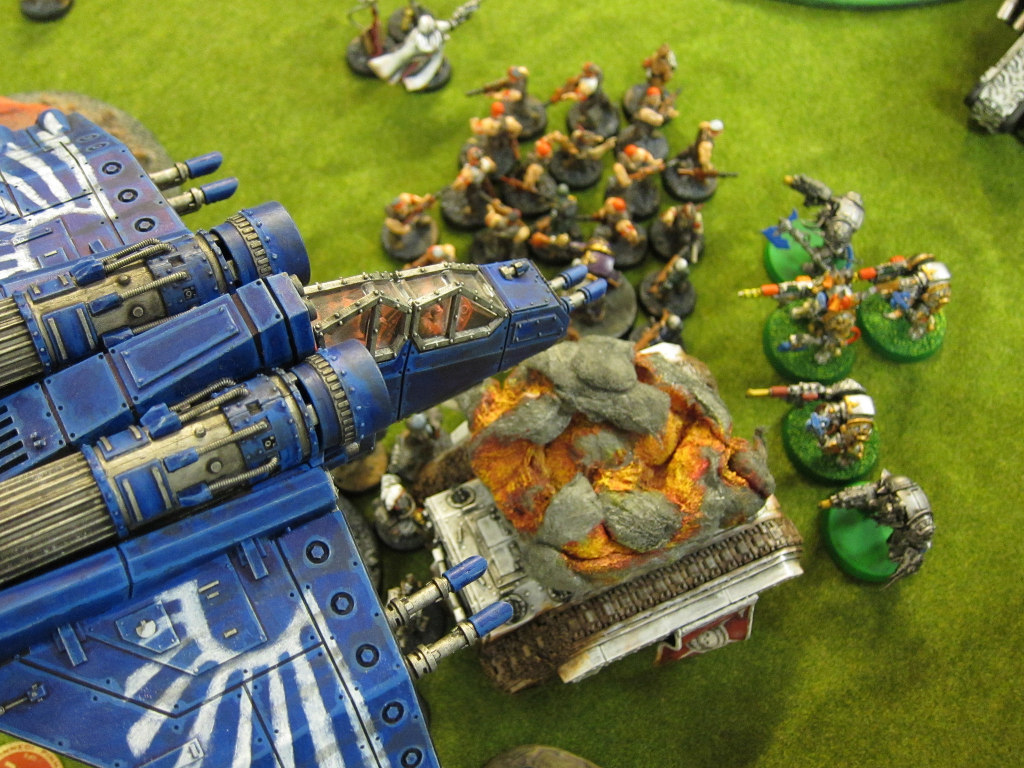
\includegraphics[height=4.5in]{pics/rob-flyer-sm}}\\
Requested air strike imminent on your position.  Take cover.
\end{minipage}
}

\vfill

\begin{columns}

  \noindent%
  Some offer nothing, others reveal the target's continent, and one
  yields their quarry's precise location.

Apply the following procedure for each of the Order and Discord cards.
Organize the numbered cards into four decks, each containing one
``Precise Location'' and two ``Clue'' cards.  Place the decks facedown
and shuffle the set.  Randomly select a deck, discarding the others
without revealing which has been selected.  Keeping the deck facedown,
add the three ``No result'' cards and shuffle the deck.  Without
revealing any contents, for each card randomly select one of its
faction's envelopes and place it inside.

The search envelopes now contain clues to and the precise location of
each alliance's objective, randomly sprinkled across the continents.
Executed carefully, even the organizer(s) won't know where the targets
will be found and may participate as players in the campaign without
compromise.

Finally, print and cut apart a set for each faction of the covert
mission cards at the end of this section.

\missionheading{Campaign Mechanics}

At the end of the three missions, Order and Discord have achieved
their campaign objective if they have discovered the precise location
of their target and control the continent it is on.  The Spoilers
achieve their campaign objective if they know the precise location of
either \emph{The Scythe} or the Magos and control that continent.
Note that the precise location might be discovered on a different
continent from the target's actual location.  This reflects the
worldwide search through ruined libraries, hacked databanks, and
captured individuals eventually yielding the location, which must then
be secured.  If a target's precise location is not found until after
the final round but the alliance ends the campaign in control of that
continent, they still achieve their campaign objective.

Following each round, Order and Discord secretly draw and keep a
search result from their respective envelopes for each continent they
control.  For each continent the Spoilers control they secretly draw
from the envelopes of both Order and Discord, record what they found,
and put the cards back.

Control of a continent is defined as the leader of the accumulated
sums for each alliance of victory points earned in matches held on
that continent.  In event of a tie, each of the tied alliances are
considered to have control.  If the Spoilers are among those tied,
they draw and return their results before the other alliances pull
from their envelopes.

\pagebreak
\missionheading{Round Pairings}

Players are paired with an opponent for each match from another
alliance as best as possible given the number of players.  Teammates
should only battle if no other set of pairings is possible.  In that
rare case, their alliance earns the lesser of the two players' victory
points.  The players though each claim their respective victory points
toward the individual rankings.

First round pairings are randomly assigned across the alliances,
optionally applying a seeding to bias toward matching players of
similar ability.  Starting with the Legions of Discord, then the
Forces of Order, and then the Spoilers, the alliances then alternate
choosing a pairing and assigning it to a continent.  The opposing
alliance responds with a table for that match.

%% (* commander's choice *)
In the second and third rounds, the alliances choose pairings.
Alternating in order by total victory points, each alliance puts
forward a continent and an unmatched player as the attacker.  The
opposing alliance with the most unmatched players in the attacker's
win/loss/draw bracket responds with a defending player and a table for
the match.  If the opposing alliances have an equal number of
unmatched players in the bracket then one alliance is randomly
selected to respond.  The defender must be chosen from the alliance's
unmatched players in the same bracket as the attacker.  If there are
no such players then the defender must be chosen from the closest
possible win/loss/draw bracket.  No two players may ever be matched
more than once.

%% (* random pairings *)
% In the second and third rounds, pairings are assigned randomly across
% the alliances within win/loss brackets as best as possible.  No two
% players may fight more than once, and opponents must be randomly
% selected from within the closest possible win/loss brackets permitting
% that, alternating shifts up and then down the brackets until a match
% is possible.  Proceeding in order by the alliances' total
% campaign-wide victory points and descending down the win/loss
% brackets, the alliances alternate choosing a pairing and assigning it
% to a continent.  The opposing alliance then responds with a table for
% that match.

%% (* tournament pairings *)
% For the second and third rounds, pairings are assigned by win/loss
% brackets as best as possible.  Process each unmatched player in order
% by number of wins, then draws if permitted by the missions, and then
% accumulated victory points.  Assign as their opponent the player from
% another alliance in the same win/draw/loss bracket with the next
% highest victory points that they have not already played.  If there
% are no such players, choose the teammate with the next highest victory
% points from the same bracket that they have not already played.  If
% there are none of those, shift the selection to the next bracket down.
%
% Once pairings are assigned, in order by total victory points the
% alliances alternate choosing a pairing and assigning it to a
% continent.  The opposing alliance then responds with a table for that
% match.

Each continent may only be assigned a limited number of matches per
round: The number of players divided by three and rounded up.  Once
that many matches have been assigned to a continent, pairings may only
be assigned to the other continents.


\missionheading{Covert Missions}

In the second and third rounds, the trailing alliances are given
covert missions to complete and make progress toward their strategic
campaign objectives despite tactical battlefield losses.

Before pairings are assigned to continents for those rounds, the
alliance with the least accumulated victory points secretly draws a
card from its covert mission deck.  Every player in that alliance may
complete the given mission objective in their match to gain the
specified bonus for their alliance.  Following the round that covert
mission is discarded and cannot be selected again, i.e., for the third
round.

In a campaign with three alliances, the middle alliance by accumulated
victory points also draws a covert mission before the second and third
rounds in the same fashion.  However, it may only be attempted by the
half of that alliance's players with the least points, rounding down.


\missionheading{Victory!}

At the conclusion of \emph{The Debacle}, an alliance has won a
campaign victory if it achieved its campaign objective and no other
alliance did as well.  An alliance that controls the majority of the
continents has won a strategic victory.  Finally, the alliance with
the greatest sum total victory points has won a tactical victory.
Each of these outcomes influences the other components of the
\emph{Caldor IV} campaign.  Celebrate the victors, but prepare for the
battles still ahead!

\end{columns}

\pagebreak
\squelchbackground

\begin{landscape}
\vspace*{-15pt}

\noindent%
\searchcard{ORDER SEARCH (1)}{Precise location:\\Apollon,\\Forge Prime.}{The
  Magos is bunkered deep in the bowels of Caldor IV's largest and
  oldest forge with his bodyguards.}\hfill%
\searchcard{ORDER SEARCH (2)}{Precise location:\\Apollon,\\North
  Starport.}{Mechanicum forces are fighting to sustain a desperate
  holdout at the complex in hopes of evacuation.}\hfill%
\searchcard{ORDER SEARCH (3)}{Precise location:\\Hermea,\\Hive
  Pargnosis.}{Witnesses cite the Magos cowering among the
  squalor and innumerable civilians of the lower hab blocks.}\hfill%
\searchcard{ORDER SEARCH (4)}{Precise location:\\Juno,\\The Scar.}{The Magos
  is leading a frantic excavation at the bottom of one of Caldor IV's
  most unnatural features.}

\vfill

\noindent%
\searchcard{ORDER SEARCH (1)}{Clue:\\Apollon.}{A planetary defense company
  saw the Magos board a ground transport near Sub-Forge
  Praxus.}\hfill%
\searchcard{ORDER SEARCH (2)}{Clue:\\Apollon.}{A small group of Skitarii,
  bodyguards of the Magos, were seen fighting on the outskirts of the
  North Starport.}\hfill%
\searchcard{ORDER SEARCH (3)}{Clue:\\Hermea.}{Shuttle pilots logged delivery
  of the Magos' entourage to the continent at the onset of the recent
  fighting.}\hfill%
\searchcard{ORDER SEARCH (4)}{Clue:\\Juno.}{A badly corrupted distress signal\\
  from the Magos' closest protege claims he was headed to The Scar.}

\vfill

\noindent%
\searchcard{ORDER SEARCH (1)}{Clue:\\Apollon.}{Entry records show the Magos
  recently interfaced with the noosphere from a terminal in Sub-Forge
  Maurus.}\hfill%
\searchcard{ORDER SEARCH (2)}{Clue:\\Apollon.}{Requisitions document that the
  Magos ordered an orbital lifter prepared but it was later
  damaged.}\hfill%
\searchcard{ORDER SEARCH (3)}{Clue:\\Hermea.}{Official records indicate the
  Magos had scheduled an oversight meeting with one of the hive
  regents.}\hfill%
\searchcard{ORDER SEARCH (4)}{Clue:\\Juno.}{The expedition's future dimming,
  of late the Magos had been obsessed with several sites in the
  wasteland.}

\vfill

\noindent%
\searchcard{ORDER SEARCH}{No result.}{The Magos' personal logs are recovered
  but are woefully outdated and yield no hint of his location.}\hfill%
\searchcard{ORDER SEARCH}{No result.}{Contact is made with a servant of the
  Magos but the line breaks before they can exchange any
  information.}\hfill%
\searchcard{ORDER SEARCH}{No result.}{None of the senior adepts still alive
  and reachable have seen or heard from the Magos in quite some
  time.}\hfill%
\searchcard{TRASH}{Throw this placeholder card away, it is not used
  in the campaign.}{Thought for the day:\\Sacrifice is best done for
  others.}

\pagebreak

\noindent%
\searchcard{DISCORD SEARCH (2)}{Precise location:\\Juno,\\The Scar.}{Scans
  show \emph{The Scythe} largely intact under mountains of dirt, but
  even if it can be uncovered, will it fly again?}\hfill%
\searchcard{DISCORD SEARCH (1)}{Precise location:\\Juno,\\House
  Etrakus.}{Entombed in rubble, a single alcove in the buried library
  is lit by shafts of light suspending a luminescent blade.}\hfill%
\searchcard{DISCORD SEARCH (3)}{Precise location:\\Hermea,\\Hive
  Pargnosis.}{Deep in the lowest sub-foundation, the mighty war engine
  has quietly powered the entire hive for eons.}\hfill%
\searchcard{DISCORD SEARCH (4)}{Precise location:\\Apollon,\\Forge
  Prime.}{\emph{The Scythe} has lain unrecognized in the Mechanicum's
  vaults for decades, a colossal failure of imagination.}

\vfill

\noindent%
\searchcard{DISCORD SEARCH (2)}{Clue:\\Juno.}{Analysis of radiation patterns
  from metals unburied across the continent point to a spectacular
  crash site.}\hfill%
\searchcard{DISCORD SEARCH (1)}{Clue:\\Juno.}{A burnt data chip plays the
  never before heard saga \emph{The Warsong of Lord Etrakus} and then
  quickly melts.}\hfill%
\searchcard{DISCORD SEARCH (3)}{Clue:\\Hermea.}{A beautiful tapestry
  allegorizes\\\emph{The Scythe} shielding Hermea's houses from
  staggering attacks.}\hfill%
\searchcard{DISCORD SEARCH (4)}{Clue:\\Apollon.}{A faded manifest for
  sub-annex~42A of the original expedition complex lists wonders
  beyond belief.}


\vfill

\noindent%
\searchcard{DISCORD SEARCH (2)}{Clue:\\Juno.}{Only something massive and
  moving incredibly fast could have ripped those gouges into the
  planet.}\hfill%
\searchcard{DISCORD SEARCH (1)}{Clue:\\Juno.}{Stone lythos from the continent
  predating the Imperium depict an illuminated warrior astride the
  world.}\hfill%
\searchcard{DISCORD SEARCH (3)}{Clue:\\Hermea.}{Early texts chart the lineage
  of the population centers back to the survivors of the founding
  houses.}\hfill%
\searchcard{DISCORD SEARCH (4)}{Clue:\\Apollon.}{An empty docking interface
  for \emph{The Scythe} is found, with Mechanicum extraction equipment
  nearby.}\hfill%

\vfill

\noindent%
\searchcard{DISCORD SEARCH}{No result.}{The long sought-for vault's\\contents
  begin crumbling immediately upon exposure to atmosphere.}\hfill%
\searchcard{DISCORD SEARCH}{No result.}{ Only false beliefs and nonsense spew
  from the hoary integrated librarian before you end his
  delusions.}\hfill%
\searchcard{DISCORD SEARCH}{No result.}{Your servants are imbeciles, useful\\
  as little more than scrap meat.}\hfill%
\searchcard{TRASH}{Throw this placeholder card away, it is not used in
  the campaign.}{Thought for the day:\\Sacrifice is best done by
  others.}

\end{landscape}

\pagebreak%

\noindent%
\covertcard%
{Interrogation}%
{Command has ordered you to capture and interrogate prisoners.  It's
  against your usual ``No mercy'' philosophy, but they're in charge.}%
{After all deployment concludes, secretly select and record an enemy
  character.  You succeed if that character is removed as a casualty
  and you pass a~D6 test against its role:

\bigskip
\begin{minipage}{1.0\linewidth}\centering
\textbf{HQ} 2+ ~~ \textbf{Elite} 3+ ~~ \textbf{Troop} 5+\\
\textbf{Fast} 4+ ~~ \textbf{Heavy} 4+  
\end{minipage}}%
{Your alliance pulls a search result for each continent on which a
  player achieved this mission as though it shared control.}
%{For each player in your alliance that passes this test, the alliance
%  of their opponent shares its search results so far with yours after
%  results are drawn this round.}%
\hfill%
\covertcard%
{Sweep \& Scan}%
{Your troops are on the roll, rapidly covering ground in the hunt for
  intel.  You might miss something moving so fast, but time's up.}%
{At the end of each of your turns beginning with Turn~2, secretly make
  a note for each primary objective marker outside your deployment
  zone which you control and have not previously controlled.  If by
  the end of the game you have controlled at least two at some point,
  you succeed.}%
{Your alliance pulls a search result for each continent on which a
  player achieved this mission as though it shared control.}

\vfill

\noindent%
\covertcard%
{Data Port}%
{You've detected an active, unsecured data port among the wreckage
  strewn about.  If you can hold it long enough, you might be able to
  extract something useful.}%
{After all deployment concludes, secretly select and record a primary
  objective marker outside your deployment zone.  You succeed if you
  control it at the end of your turn for any two turns in a row,
  excluding Turn~1.}%
{In addition to the points you earn as usual, your alliance gains half
  the maximum victory points possible for this match toward its
  overall and this continent.} \hfill%
\covertcard%
{Signals}%
{You're tracking an enemy HQ signal.  If you can triangulate it,
  you'll know where they're based.}%
{After all deployment concludes, secretly select and record a table
  quarter not on your table edge.  At game end if you have a scoring
  unit in that quarter and your opponent does not, you succeed.  Units
  with Objective Secured trump those without.}%
{In addition to the points you earn as usual, your alliance gains half
  the maximum victory points possible for this match toward its
  overall and this continent.}

\pagebreak
\restorebackground%

%\vfill
%\noindent%
%\begin{minipage}[t]{1.0\linewidth}\centering\small\it%
%\fbox{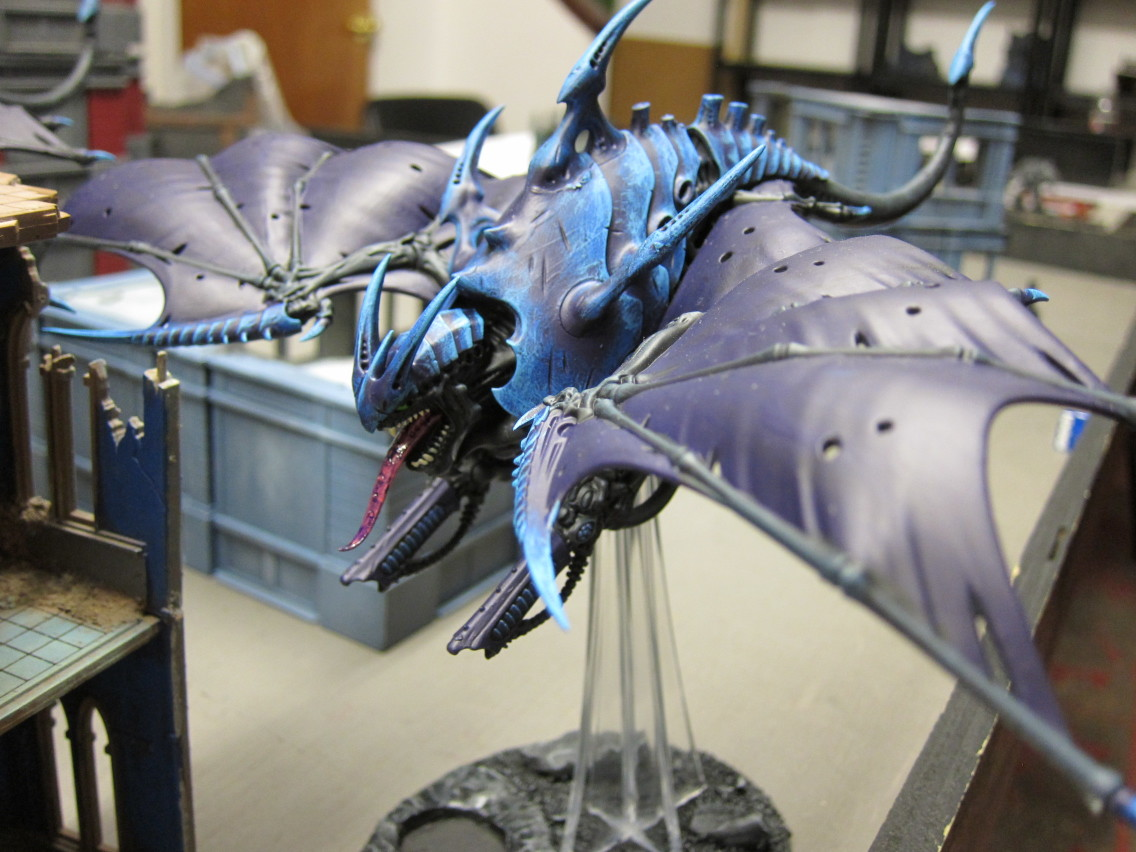
\includegraphics[width=(1.0\linewidth)]{pics/IMG_9230-sm}}\\
%Scour the skies!
%\end{minipage}
